\documentclass[11pt]{article}
\usepackage[final]{acl}
\usepackage{times}
\usepackage{latexsym}
\usepackage[T1]{fontenc}
\usepackage[utf8]{inputenc}
\usepackage{microtype}
\usepackage{graphicx}
\usepackage{booktabs}
\usepackage{amsmath}
\usepackage{url}

\graphicspath{{figs/}}

\title{It Was the GPU, Not the Algorithm: Controlling for Hardware\\
Variance When Speedrunning GPT-2 Training on a Shared Cluster}

\author{Jan Kadlec \\
  Faculty of Electrical Engineering \\
  Czech Technical University in Prague \\
  \texttt{kadlej27@student.cvut.cz} \\}

\begin{document}
\maketitle

\begin{abstract}
We attempt the BottleCapAI ``no-cap'' GPT-2 efficiency benchmark---train a
124M-parameter model to a fixed validation loss as \emph{fast} as
possible---without dedicated hardware, on the shared MetaCentrum academic HPC
cluster. Across 43 logged runs we evaluate three efficiency ideas: sliding-window
attention, log-frequency bias initialisation, and explicitly forced
FlashAttention. Our headline finding is methodological rather than algorithmic:
because the cluster scheduler assigns a heterogeneous, non-deterministic mix of
GPUs, the wall-clock time of the \emph{identical} training job varies by
$4.8\times$ (2.4\,h on an H100 to 11.5\,h on an A40), completely swamping any
algorithmic speedup, which we bound at $\le\!0.2\%$ on matched hardware. To
recover fair comparisons we build an open-source dashboard that filters and
groups Weights \& Biases runs by GPU model---a dimension W\&B records but does
not expose as a first-class filter. With hardware held constant the algorithmic
verdicts are clean negatives: sliding-window attention monotonically worsens
loss \emph{and} runs slower; forcing FlashAttention is a no-op because PyTorch's
attention kernel already uses it; log-frequency init helps only at the level of
run-to-run noise. We argue that speedrun results on shared clusters are
meaningless unless reported against a same-hardware baseline.
\end{abstract}

\section{Introduction}

The BottleCapAI benchmark~\cite{bottlecap2025}, a single-GPU fork of Keller
Jordan's \texttt{modded-nanogpt} speedrun~\cite{jordan2024moddednanogpt}, poses a
deliberately narrow question: starting from a fixed 124M-parameter GPT-2
baseline, can an \emph{algorithmic} idea reach a validation loss of
$3.3821$ on a subset of FineWeb~\cite{penedo2024fineweb} in less wall-clock time?
The rules explicitly discourage hyperparameter tuning and hardware-specific
micro-optimisation; the metric of merit is time-to-target.

This framing assumes a fixed, dedicated GPU. We did not have one. Like many
students, we ran on MetaCentrum, a shared PBS cluster where the scheduler hands
out whatever accelerator is free within a requested capability class. The
consequence is the central problem of this paper: \emph{the independent variable
of the benchmark---time---is dominated by a confound we do not control}, namely
which physical GPU the job lands on.

We make four contributions. (1) We implement and evaluate three efficiency ideas
on top of the baseline (\S\ref{sec:experiments}). (2) We quantify the hardware
confound: the identical job varies $4.8\times$ in wall-clock across six GPU
models, and even $1.4\times$ within a single model (\S\ref{sec:confound}). (3) We
release an open dashboard that makes ``GPU model'' a first-class filter over W\&B
runs, which is what makes any of the algorithmic comparisons interpretable
(\S\ref{sec:dashboard}). (4) We report honest negative results and a short set of
methodological recommendations for speedrunning on shared infrastructure
(\S\ref{sec:discussion}). Negative results are explicitly solicited by the
benchmark, and we think the methodological point generalises well beyond it.

\section{Setup}
\label{sec:setup}

\paragraph{Model and baseline.} The baseline is a pre-norm GPT-2 small
(\texttt{d12}: 12 layers, 12 heads, $d{=}768$) with rotary position
embeddings~\cite{su2021roformer}, RMSNorm~\cite{zhang2019rmsnorm}, tied input/output
embeddings~\cite{press2017tying}, and no biases. It is trained in bfloat16 with
\texttt{torch.compile} and AdamW~\cite{loshchilov2019adamw} for 4768 steps at an
effective batch of $512\times1024$ tokens (micro-batch 16, gradient accumulation
32, sequence length 1024), i.e.\ $\approx\!2.5$B tokens. Attention uses PyTorch's
fused \texttt{scaled\_dot\_product\_attention} (SDPA). All hyperparameters are held
at the baseline values throughout; we change only the algorithmic factor under test.

\paragraph{Cluster.} MetaCentrum exposes GPUs through PBS resource selectors
(e.g.\ \texttt{gpu\_cap}). A request such as \texttt{gpu\_cap=compute\_80}
matches any Ampere-or-newer device, so a single job specification can run on an
A40, L40S, A100, H100, or RTX~PRO~6000 depending on availability. We log every
run to W\&B~\cite{biewald2020wandb}, which records the assigned GPU in run
metadata.

\paragraph{Runs.} We analyse all 43 runs in our W\&B project (42 finished, 1
crashed), spanning six distinct GPU models. Unless noted, ``wall-clock'' is the
W\&B process runtime on the compute node, which includes periodic validation.

\section{The Hardware Confound}
\label{sec:confound}

We first measure the baseline configuration---no algorithmic change---wherever the
scheduler happened to place it. Table~\ref{tab:gpu} and Figure~\ref{fig:gpu} show
the result. The same 4768-step job takes 2.4\,h on an H100 and 9.3\,h on an A40
\emph{on average}; the single fastest and slowest baseline runs differ by
$4.8\times$ (8{,}570\,s vs.\ 41{,}453\,s). Crucially the variance is not only
across models: two A40 runs of the identical job differ by $40\%$ (29.5k vs.\
41.5k\,s), presumably from node-level contention and thermals.

\begin{table}[t]
\centering
\small
\begin{tabular}{lrrr}
\toprule
GPU & $n$ & wall-clock & val.\ loss \\
\midrule
H100 NVL              & 1  & 2.38\,h & 3.378 \\
RTX PRO 6000 Blackw.  & 1  & 2.62\,h & 3.381 \\
A100-SXM4-40GB        & 3  & 3.93\,h & 3.379 \\
L40S                  & 12 & 5.24\,h & 3.381 \\
A40                   & 3  & 9.33\,h & 3.380 \\
\midrule
\multicolumn{2}{l}{slow / fast ratio} & $4.84\times$ & --- \\
\bottomrule
\end{tabular}
\caption{The \emph{identical} baseline job across GPUs. Wall-clock spans
$4.8\times$ while validation loss is invariant within $\pm0.0015$.}
\label{tab:gpu}
\end{table}

\begin{figure}[t]
\centering
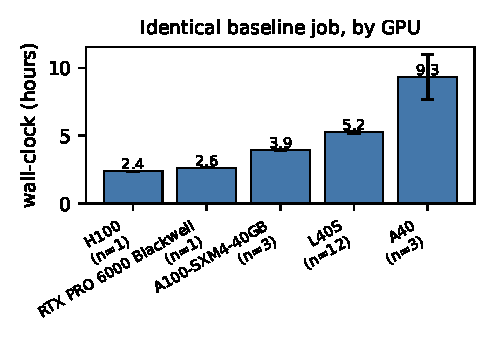
\includegraphics[width=0.78\columnwidth]{fig_gpu_walltime}
\caption{Wall-clock of the identical baseline job by GPU model. Error bar shows
the within-model min--max for the A40.}
\label{fig:gpu}
\end{figure}

Two things follow. First, validation loss is essentially \emph{invariant} to the
GPU: every baseline run lands at $3.380\pm0.0015$, as expected---the optimisation
trajectory does not depend on the silicon, only its speed. The standard deviation
of validation loss across the 20 baseline runs is $0.00146$; we treat
$\pm0.0015$ as the run-to-run \emph{noise floor} for the rest of the paper.
Second, and decisively: a hypothetical algorithmic speedup of even 10\% is a
$\sim$0.5\,h effect on an L40S, whereas merely being rescheduled from an L40S to
an A40 is a $+4$\,h effect. \textbf{Any speedup smaller than the inter-GPU spread
is unmeasurable unless hardware is held constant.} This is the motivation for
everything that follows.

\section{A Dashboard to Control for Hardware}
\label{sec:dashboard}

W\&B is excellent at grouping runs by anything in the logged \emph{config}
(learning rate, model size, \dots), but the GPU model lives in per-run
\emph{system metadata}, which the standard run table does not surface as a
groupable or filterable column. To compare two algorithmic variants fairly we
therefore need to first restrict attention to runs that share a GPU---a query the
native UI makes awkward.

We built a small open-source dashboard for exactly this.\footnote{Source:
\url{https://github.com/Pokrt/wandb-dashboard}; live:
\url{https://gpt-dashboard.jan-kadlec.cz}.} A FastAPI backend wraps the W\&B public
API with a short-TTL in-memory cache and extracts the GPU name from each run's
metadata, exposing endpoints to list the distinct GPUs in a project
(\texttt{/runs/gpus}), filter runs by GPU substring, status, date, or training
command (\texttt{/runs?gpu=\dots}), and fetch multiple runs' loss histories in
parallel for overlay (\texttt{/runs/compare/metrics}). A Nuxt/Vue frontend with
Chart.js/ECharts renders the loss curves and lets the user pin a GPU model before
comparing. Selecting, say, ``A40'' collapses the dataset to same-hardware runs and
makes an A/B between two algorithms meaningful. All figures and tables in
\S\ref{sec:experiments} are produced under exactly this same-GPU discipline.

\section{Algorithmic Experiments}
\label{sec:experiments}

Each idea is compared against the baseline \emph{on the same GPU model}, so that
the residual difference is attributable to the algorithm rather than the
scheduler.

\subsection{Sliding-Window Attention}

\paragraph{Idea.} Restrict each token to attend only to the previous $w$ tokens,
as in Longformer~\cite{beltagy2020longformer} and Mistral~\cite{jiang2023mistral}.
Asymptotically this turns the $O(T^2)$ attention into $O(Tw)$, which should help
both speed and memory at long context. We implement it by intersecting the causal
mask with a band of width $w$ and passing the result as an additive
\texttt{attn\_mask} to SDPA, testing $w\in\{64,128,256\}$ against full causal
attention.

\paragraph{Result (negative, twice over).} Figure~\ref{fig:swa} and
Table~\ref{tab:algo} show a clean monotonic degradation: smaller windows give
strictly worse validation loss at the fixed step budget ($3.380\to3.399\to3.441
\to3.498$ for full$\to$256$\to$128$\to$64), far outside the noise floor. At
$T{=}1024$ a 124M model evidently needs global context to hit the target. Worse,
sliding-window attention was also \emph{slower}: on the L40S it took
5.8--6.0\,h versus 5.2\,h for full attention. The reason is implementation-level
but instructive---supplying an explicit floating-point \texttt{attn\_mask}
disables SDPA's fused causal-attention fast path and falls back to a slower
kernel. The ``efficient'' variant was thus both less accurate and less efficient.

\begin{figure}[t]
\centering
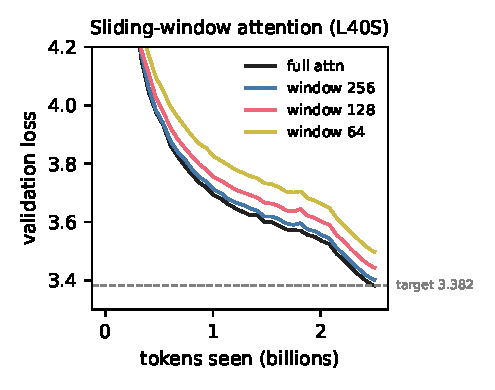
\includegraphics[width=0.82\columnwidth]{fig_swa_curves}
\caption{Validation loss vs.\ tokens for sliding-window attention, all on the
same GPU (L40S). Smaller windows are uniformly worse; only full attention reaches
the target.}
\label{fig:swa}
\end{figure}

\subsection{Forced FlashAttention}

\paragraph{Idea.} FlashAttention~\cite{dao2022flashattention,dao2023flashattention2}
is an IO-aware exact-attention kernel with $O(T)$ memory. We added a flag that
wraps SDPA in \texttt{sdp\_kernel(enable\_flash=True, enable\_math=False,
enable\_mem\_efficient=False)} to force the flash backend.

\paragraph{Result (no-op).} On matched A100s the forced-flash runs were within
$0.2\%$ of baseline wall-clock (3.92\,h vs.\ 3.93\,h) and within the noise floor
on loss (Table~\ref{tab:algo}). The reason is that \emph{the baseline already
runs FlashAttention}: PyTorch's SDPA is a dispatcher that automatically selects a
fused flash/memory-efficient kernel for causal attention on Ampere-and-newer
hardware, and every GPU in our pool (A40, L40S, A100, H100, RTX~PRO~6000) is
Ampere or newer. Forcing the backend therefore changes nothing the baseline was
not already doing. We note candidly that we did not initially realise SDPA
defaults to FlashAttention; the entire ``add flash attention'' effort amounted, in
hindsight, to re-enabling a kernel that was already on---exactly the kind of
phantom optimisation that careful, hardware-controlled measurement is meant to
expose.\footnote{This was compounded by an implementation detail. An earlier code
path enabled the third-party \texttt{flash-attn} package automatically whenever it
imported successfully (with no flag), and four runs were launched with it. The
package never built on the cluster---its ${\sim}1$\,h source compile and
${\sim}10$\,GB footprint exhausted the scratch quota---so the \texttt{try/except}
import silently fell back to SDPA. The W\&B-captured \texttt{pip freeze} for all
four runs confirms \texttt{flash\_attn} was absent, and their wall-clock matches
the SDPA baselines on the same GPU to within noise. No run in the project ever
executed the standalone library.}

\subsection{Log-Frequency Bias Initialisation}

\paragraph{Idea.} At initialisation a softmax language model with a uniform output
layer assigns probability $1/V$ to every token, for an initial loss of
$\log V \approx 10.8$. If instead we set the output-layer bias to the log unigram
frequencies of the training corpus, $b_i = \log\hat{f}_i$, the model's
initial distribution \emph{is} the unigram distribution and the network only has
to learn deviations from it. We estimate $\hat f_i$ from the training shards with
Laplace smoothing ($\varepsilon{=}1$) to avoid $\log 0$:
\[
\hat f_i = \frac{c_i + \varepsilon}{\sum_j (c_j + \varepsilon)} .
\]
This adds a learnable bias to the otherwise bias-free, weight-tied output layer
and costs one pass over the token counts at startup.

\begin{figure}[t]
\centering
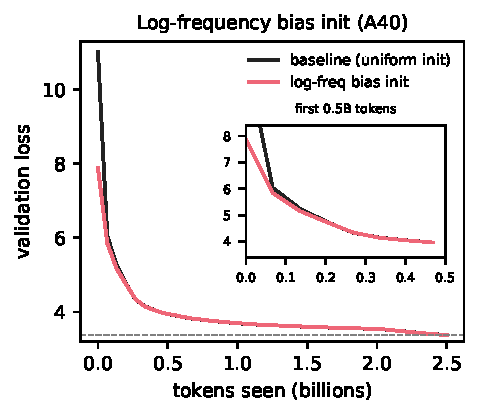
\includegraphics[width=0.82\columnwidth]{fig_logfreq}
\caption{Log-frequency bias init vs.\ baseline on the same GPU (A40). The bias
gives a ${\sim}3$-nat head start at initialisation (7.9 vs.\ $\log V\!\approx\!11.0$),
but the baseline learns the unigram marginal within the first ${\sim}0.2$B tokens
(inset) and the curves are indistinguishable thereafter.}
\label{fig:logfreq}
\end{figure}

\paragraph{Result (early head start, no lasting gain).} The bias does exactly
what it should \emph{at initialisation}: validation loss starts at $7.9$ rather
than the baseline's $11.0$ (the uniform-init value $\log V$), a head start of
${\sim}3$ nats (Figure~\ref{fig:logfreq}). But this is precisely the easiest thing
for the model to learn---the baseline matches the unigram marginal within the
first ${\sim}0.2$B tokens (a few hundred steps), after which the two trajectories
are indistinguishable. The head start therefore buys early-step loss, not final
loss or wall-clock. On matched A40s the final validation loss was $3.379$ versus
$3.380$ for baseline---an improvement of $0.0015$, exactly one noise-$\sigma$.
Suggestively, the single best validation loss across all 43 runs ($3.3758$) is a
log-frequency run, and the direction is consistent, but we cannot claim
significance at this sample size. The intervention is essentially free and
theoretically well-motivated, so it is a reasonable default; it is not a speedup.

\begin{table}[t]
\centering
\small
\begin{tabular}{llrr}
\toprule
GPU & Variant & wall-clock & val.\ loss \\
\midrule
L40S & full attn (base)   & 5.24\,h & 3.380 \\
L40S & window 256         & 5.93\,h & 3.399 \\
L40S & window 128         & 6.00\,h & 3.441 \\
L40S & window 64          & 5.79\,h & 3.498 \\
\midrule
A100 & baseline           & 3.93\,h & 3.379 \\
A100 & forced flash       & 3.92\,h & 3.383 \\
\midrule
A40  & baseline           & 9.33\,h & 3.380 \\
A40  & log-freq init      & 8.90\,h & 3.379 \\
\bottomrule
\end{tabular}
\caption{Algorithmic variants, each compared to baseline \emph{on the same GPU
model}. Differences in loss below $\pm0.0015$ are within the noise floor; the
A40 wall-clock difference reflects scheduler variance, not the algorithm.}
\label{tab:algo}
\end{table}

\section{Discussion}
\label{sec:discussion}

\paragraph{What the experiment actually surfaced.} Beyond the three
ideas, most of our effort went into problems that have nothing to do with
language modelling: a command-line \texttt{qsub -l select=\dots} silently
overriding the in-script resource directive and dropping \texttt{scratch\_local},
causing out-of-disk failures; Kerberos tickets preventing non-interactive job
submission; the \texttt{flash-attn} build blowing the scratch quota; and unstable
relative paths on compute nodes. These are mundane, but they are the real cost of
``free'' shared compute and the reason careful logging mattered.

\paragraph{Recommendations.} (1) On a shared cluster, \emph{never} report a
speedup without a same-hardware baseline; the inter-GPU spread here ($4.8\times$)
is two orders of magnitude larger than any algorithmic effect we could produce.
(2) Where possible, pin the node (PBS \texttt{vnode=}) or, better, run baseline
and variant as a \emph{pair} inside one allocation so they share the exact device.
(3) Always log the GPU model and make it a first-class filter dimension---this is
the single change that turned our otherwise uninterpretable run table into the
controlled comparisons above. (4) Treat ``obvious'' efficiency wins skeptically:
forcing FlashAttention was redundant with the framework, and shrinking the
attention window cost both accuracy and speed.

\paragraph{Limitations.} Some cells (H100, RTX~PRO~6000) have $n{=}1$ because the
scheduler rarely assigned those devices; our within-model variance estimate is
strongest for the A40 and L40S. We did not retune hyperparameters for the
algorithmic variants by design, so e.g.\ sliding-window attention might fare
better with a compensating longer context or step budget---but that would change
the controlled comparison. Statistical power for the log-frequency effect is
limited by the cost of repeated multi-hour runs.

\section{Conclusion}

We set out to speed up GPT-2 training and instead learned that, on a shared
cluster, the dominant variable is the one the benchmark assumes away: the GPU.
Quantifying that confound, building tooling to control for it, and re-evaluating
three efficiency ideas against same-hardware baselines turned a set of
inconclusive runs into clear conclusions---all negative or neutral, but
trustworthy. The transferable lesson is simple: a wall-clock speedup is only as
credible as the baseline it is measured against, and on heterogeneous
infrastructure that baseline must run on the same chip.

\section*{Reproducibility and Resources}

Training code, job scripts, and session logs:
\url{https://github.com/Pokrt/NoCap-Test}. GPU-aware W\&B dashboard:
\url{https://github.com/Pokrt/wandb-dashboard}
(\url{https://gpt-dashboard.jan-kadlec.cz}). All numbers are computed from the 43
runs in the W\&B project \texttt{benchmark\_gpt2}.

\bibliography{refs}

\end{document}
